\documentclass[a4paper,12pt]{article}
\usepackage{xcolor}
\usepackage{etoc}
\usepackage{soul}
\usepackage{blindtext}
\usepackage{scrextend}
\usepackage[utf8]{inputenc}
\usepackage[USenglish,british,american,australian,english]{babel}
\usepackage{helvet}
\usepackage{graphicx}
\usepackage{color}
\usepackage{geometry}
\usepackage{regexpatch,fancyvrb,xparse}
\usepackage{listings}
\usepackage{hyperref}
\hypersetup{
    colorlinks,
    citecolor=black,
    filecolor=black,
    linkcolor=black,
    urlcolor=black
}
\lstset{
    frame=tb, % draw a frame at the top and bottom of the code block
    tabsize=4, % tab space width
    showstringspaces=false, % don't mark spaces in strings
    numbers=left, % display line numbers on the left
    commentstyle=\color{green}, % comment color
    keywordstyle=\color{blue}, % keyword color
    stringstyle=\color{red} % string color
}


\makeatletter
\let\do@footnotetext\@footnotetext
\regexpatchcmd{\do@footnotetext}
  {\c{insert}\c{footins}\cB.(.*)\cE.}
  {\1\c{egroup}}
  {}{}
\def\@footnotetext{\insert\footins\bgroup\@makeother\#\do@footnotetext}
\newcommand{\ttvar}{\begingroup\@makeother\#\@ttvar}
\newcommand{\@ttvar}[1]{\ttfamily\detokenize{#1}\endgroup}
\makeatother
\newcommand\tab[1][1cm]{\hspace*{#1}}
\geometry{hmargin={2cm, 2cm}, height=10.0in}

\begin{document}
\thispagestyle{empty}
%% ------------------------ NAGLOWEK STRONY ---------------------------------

\includegraphics[height=37.5mm]{agh_nzw_a_en_1w_wbr_pms}\\
\rule{30mm}{0pt}{
{\large \textsf{Faculty of Physics and Applied Computer Science}}\\
\rule{\textwidth}{3pt}\\
\rule[2ex]
{\textwidth}{1pt}\\
\vspace{7ex}
\begin{center}
{\LARGE \bf \textsf{Engineering thesis}}\\
\vspace{13ex}
% --------------------------- IMIE I NAZWISKO -------------------------------
{\bf \Large \textsf{Michal Stefaniuk}}\\
\vspace{3ex}
{\small \sf major: {\bf \textsf{applied computer science}}}\\
\vspace{1.5ex}
%{\small \sf specialisation: {\bf \textsf{software engineering}}}\\
\vspace{10ex}
%% ------------------------ TYTUL PRACY --------------------------------------
{\bf \huge \textsf{Web application developement using WebToolkit
C++ on the example of a banking service}}\\
\vspace{14ex}
%% ------------------------ OPIEKUN PRACY ------------------------------------
{\Large \sf Supervisor: {\bf \textsf{Dr Grzegorz Gach}}}\\
\vspace{22ex}
{\large \bf \textsf{Cracow, June 2021}}
\end{center}
%% =====  STRONA TYTULOWA PRACY MAGISTERSKIEJKIEJ ====

\newpage

\begin{center}
	{\bf\large\textsf{Oświadczenie studenta}}\\
\end{center}

%% ===== PL TYL STRONY TYTULOWEJ PRACY MAGISTERSKIEJKIEJ ====
{Uprzedzony(-a) o odpowiedzialnosci karnej na podstawie art. 115 ust. 1 i 2 ustawy z dnia 4 lutego 1994 r. o prawie autorskim i prawach pokrewnych (t.j. Dz. U. z 2018 r. poz. 1191 z pozn. zm.): ,,Kto przywlaszcza sobie autorstwo albo wprowadza w blad co do autorstwa calosci lub czesci cudzego utworu albo artystycznego wykonania, podlega grzywnie, karze ograniczenia wolnosci albo pozbawienia wolnosci do lat 3. Tej samej karze podlega, kto rozpowszechnia bez podania nazwiska lub pseudonimu tworcy cudzy utwor w wersji oryginalnej albo w postaci opracowania, artystyczne wykonanie albo publicznie znieksztalca taki utwor, artystyczne wykonanie, fonogram, wideogram lub nadanie.", a takze uprzedzony(-a) o odpowiedzialnosci dyscyplinarnej na podstawie art. 307 ust. 1 ustawy z dnia 20 lipca 2018r. Prawo o szkolnictwie wyzszym i nauce (Dz. U. z 2018 r. poz. 1668 z pozn. zm.) ,,Student podlega odpowiedzialnosci dyscyplinarnej za naruszenie przepisow obowiazujacych w uczelni oraz za czyn uchybiajacy godnosci studenta.", oswiadczam, ze niniejsza prace dyplomowa wykonalem(-am) osobiscie i samodzielnie i nie korzystalem(-am) ze zrodel innych niz wymienione w pracy.

\bigskip

Jednoczesnie Uczelnia informuje, ze zgodnie z art. 15a ww. ustawy o prawie autorskim i prawach pokrewnych Uczelni przysluguje pierwszenstwo w opublikowaniu pracy dyplomowej studenta. Jezeli Uczelnia nie opublikowala pracy dyplomowej w terminie 6 miesiecy od dnia jej obrony, autor moze ja opublikowac, chyba ze praca jest czescia utworu zbiorowego. Ponadto Uczelnia jako podmiot, o ktorym mowa w art. 7 ust. 1 pkt 1 ustawy z dnia 20 lipca 2018 r. Prawo o szkolnictwie wyzszym i nauce (Dz. U. z 2018 r. poz. 1668 z po 'zn. zm.), moze korzystac bez wynagrodzenia i bez koniecznosci uzyskania zgody autora z utworu stworzonego przez studenta w wyniku wykonywania obowiazkow zwiazanych z odbywaniem studiow, udostepniac utwor ministrowi wlasciwemu do spraw szkolnictwa wyzszego i nauki oraz korzystac z utworow znajdujacych sie w prowadzonych przez niego bazach danych, w celu sprawdzania z wykorzystaniem systemu antyplagiatowego. Minister wlasciwy do spraw szkolnictwa wyzszego i nauki moze korzystac z prac dyplomowych znajdujacych sie w prowadzonych przez niego bazach danych w zakresie niezbednym do zapewnienia prawidlowego utrzymania i rozwoju tych baz oraz wspolpracujacych z nimi systemow informatycznych.}\\

\bigskip

\newpage
\tableofcontents

\section*{Introduction}
\addcontentsline{toc}{section}{\protect\numberline{}Introduction}%
\tab {Software engineering is a very wide area of engineering which particularly concerns developing and maintaining programming products. A development process itself is a major challenge to all people involved, starting with engineers creating the code, continuing with product owners who are managing teams and coordinating the work flow and ending-up with managers who are setting the direction of the whole process.

\bigskip
The main motivation to create this thesis was simply to present a development process that includes basic and nowadays necessary tools which are significantly helpful in such process. Simultaneously creating a C++ web application was an equally important factor. To carry out the development and present all tools it was decided that an example C++ web application will be created with a GUI library in modern C++ called \textbf{Web Toolkit}. 

\bigskip 
Nowadays in a software engineering world there is a trend to migrate desktop applications to the internet, which has also impacted a lot GUI desktop libraries in decreasing their utilities. The secondary reason behind choosing C++ to create a web application, which is quite unusual, was to show the tremendous possibilities that this language still provides and to exhibit the capabilities of open source libraries shared among developers and engineers. The bottom line is - next chapters are a review of possibilities that C++-based web library provides.

\
}
\newpage
\section{Projects assumptions}

\subsection{Application's blue-print}
{\tab The application is a single-page service run on a local server with an \textbf{http://localhost:8080/} address. After starting, logging panel appears, giving the user an opportunity to type their credentials and log-in. 

\bigskip
The idea of the service is to provide basic functionalities of a banking service like for instance transferring money or checking their balance to the user. These required implementation of secure back-end layer with a database containing information about the users and transactions and a front-end layer which is transparent to the user. 

\bigskip
Regarding the credentials a user will see different features after logging into the service. There might be many accounts created and held up in the database of the service but there are only two rights of access.}\\
\begin{labeling}{alligator}
\item [\textbf{USER}] Transferring money and seeing current account's balance.
\item [\textbf{ADMIN}] Seeing details about every account in the service as well as having access to the logs from the application.
\end{labeling}

\bigskip
After user decides to quit the service, a possibility of logging out is provided and whilst doing that the application returns to the logging page where session is refreshed and database is updated. If the user was an administrator of the service, an access to the console logs that are gathering and sniffing network traffic like HTTP methods for RESTful APIs is also granted.  

\subsection{Programming environment}
{\tab Developing any kind of programs usually requires specific environmental variables therefore a programmer's task is to choose a specific set of tools which will be the most handy during the process.  

\bigskip
Regarding the specifics of the project, the chosen set of tools looks like following:
\begin{labeling}{alligator}
\item [\textbf{IDE}] Microsoft Visual Studio Community 2019,
\item [\textbf{LIBRARY}] Web Toolkit 4.3.1,
\item [\textbf{LIBRARY}] Boost C++ lib [latest version],
\item [\textbf{TOOL}] CMake VERSION 2.4,
\item [\textbf{TOOL}] Git BASH.
\end{labeling}}

The application was developed under Windows 10 64-bit operating system, but it could have been developed under any other platform that is supported by WebToolkit library.

\newpage
\subsubsection*{IDE - Integrated Development Environment}
{
\tab IDE is a program or a set of programs merged into one that usually gathers tools, libraries, debuggers, run time scripts and any other stuff necessary for the developer to write the code. The purpose of IDE is to allow easily and swiftly create code, but at the same time test it, compile it and run it in one place. 

\bigskip
The advantage of this solution is that it gives the developer an opportunity to set up and scale his development environment adjusting it to the project needs. Usually IDE, as well as modern text editors, also support plugins which are nice addition to the program, like for instance syntax highlighters, semantics hints, code analyzers or refactoring scripts.

\bigskip
The chosen IDE for this project is \textbf{Microsoft Visual Studio Community 2019}. Web Toolkit library is supported on various platforms including Linux distributions (even less popular ones like ArchLinux, Slackware or Opensuse), Windows or other operating systems like Android, Raspberry Pi or even OS X. The consequence of choosing MSV IDE was using Windows platform and prebuilt Windows binaries of the WT library.

\bigskip
\textbf{Microsoft Visual Studio} is and IDE produced by Microsoft Company and it allows creating cross-platform software with graphical user interface. It basically supports every programming language but the basic package contains support for 
\begin{itemize}
	\item Microsoft Visual C\ttvar{#}
	\item Microsoft Visual C++
	\item Microsoft Visual Basic
	\item Microsoft Visual J\ttvar{#}
	\item Microsoft Visual Web Developer ASP.NET
	\item Microsoft Visual F\ttvar{#}
\end{itemize}

MSVC also provides a lot of built-in features. A lot of them occurred to be significantly useful in the process of developing this application. A few most important ones are
\begin{itemize}
	\item Debugger, Linker and Compiler
	\item Projects and Build Systems
	\item Writing and refactoring C++ code
	\item Code analysis overview
	\item Unit tests support
	\item Universal Windows Apps like command line appliactions
\end{itemize}

}

\subsubsection*{Boost C++ library}
{
\tab Boost is a collection of C++ libraries that enhances capabilities of C++ code development, which is also licensed by \textbf{Boost Software License}. For the project Boost is necessary to build Web Toolkit library as it's implementation uses Boost functionalities.

\bigskip
The most important features provided by Boost are
\begin{itemize}
	\item Algorithms
	\item Concurrent programming
	\item Complex containers
	\item Correctness validating and enhanced unit testing
	\item Additional data structures (like bimap, fusion, tuple etc)
	\item High level programming and functional objects
	\item Parsers and graphs
	\item Meta-programming with templates
\end{itemize}
	
Boost library as a collection is not used in this project explicitly, as the application was developed in Microsoft Visual Studio environment with pre-built Windows binaries. However, for automation server, the project is built under linux machine where WebToolkit needs to be built manually, therefore boost is required. More details will be unveiled in "Automation server" chapter.
}
\subsubsection*{CMake}
{
\tab CMake is a cross platform tool that provides automatic management of compiler that builds the code of an application. It's role is to create a configuration for project files of popular programming environments, which then are used in a process of compilation. The main advantage of using CMake is it's independence of the compiler and the platform. However CMake as a standalone program creates files with rules for compilation dedicated to another program like IDE and it forms a unified building environment. CMake stands for \textit{Cross-platform Make}.

\bigskip
The most important features provided by CMake are
\begin{itemize}
	\item Platform independence
	\item Cross compilation
	\item Out-of-source building
	\item Building projects with complex catalog structure 
	\item Unit testing support
	\item Detecting dependencies and outer libraries
\end{itemize}
This project required including CMake tool because of various dependencies and complex building due to including Web Toolkit and Boost.  

\bigskip
To be able to explore favors that CMake offers one must create \textbf{CMakeLists.txt} file placed in the main catalog of the project. The core of this file is a simple scripting language that describes rules and defines variables telling the compiler how to link files and what should be the outcome of the compilation process.

\bigskip
Let's have an example project\cite{cmakeintroduction} which structure looks like below\newline
\begin{lstlisting}[frame=single, language=C++, caption={Example CMake project structure}, captionpos=b]
 .
 |-- CMakeLists.txt
 |-- build
 |-- include
 |   \-- Student.h
 \-- src
     |-- Student.cpp
     \-- mainapp.cpp
\end{lstlisting}

\bigskip
The content of \textbf{*.cpp} and \textbf{*.h} files is irrelevant here, at this point it could be any code. In the main directory we have a simple \textbf{CMakeLists.txt} which is used to build the project. The code of our CMakeLists script:\newline

\begin{lstlisting}[frame=single, language=C++, caption={CMakeLists.txt of example project}, captionpos=b]
cmake_minimum_required(VERSION 2.8.9)
project(directory_test)

#Bring the headers, such as Student.h into the project
include_directories(include)

#Can manually add the sources using the set command as follows:
#set(SOURCES src/mainapp.cpp src/Student.cpp)

#However, the file(GLOB...) allows for wildcard additions:
file(GLOB SOURCES "src/*.cpp")

add_executable(testStudent ${SOURCES})
\end{lstlisting}
\bigskip
The most important things that above CMake will perform (in order from the top) are
\begin{itemize}
	\item Include directories to let the CMake know where headers files with definitions are
	\item Sources are also set, but the line is commented out as each file needs to be manually added in place
	\item file() command to add source files to project's GLOB SOURCES
	\item add\_executable() which uses SOURCES variable in order to build executable program
\end{itemize}


\noindent Now to invoke building using CMake:
\begin{lstlisting}[language=bash]
  $ mkdir build && cd build
  $ cmake ..
  $ make
  $ ./testStudent
\end{lstlisting}
  
\bigskip Commands above will create \hl{build} directory. From there cmake will create \textbf{Makefile} containing references to all sources and headers, which ultimately will create an executable that is ready to be run. This as a very basic example of how \textbf{CMake} works. In next chapters there will be more details about \textbf{CMake} and what is the main concept behind basing on the one used in project. 

}

\subsubsection*{Others}
\textit{Git BASH} tool and \textit{Web Toolkit} library are described thoroughly in next chapters.
\newpage

\section{WebToolkit C++ library}
\subsection{Library overview}
{\tab \textbf{Web Toolkit} is an open-source C++ library that allows developers to create SAP web applications without writing single line of JavaScript code. The main concept behind \cite{singlepageapplications}SAP (\hl{Single Page Applications}) is they do not render HTML files, but instead they use asynchronous JavaScript (AJAX) to reload contents of the page in real time without refreshing the whole page. To some extent it might be a bit misleading, as with loading different content, the URL of the page changes as well, like in ordinary multi-page service.

\begin{figure}[h]
  \centering
    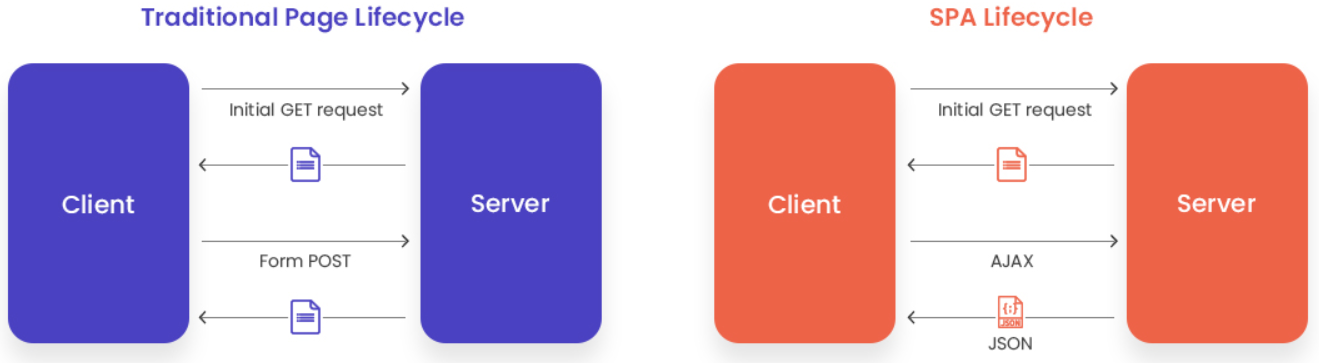
\includegraphics[width=1.0\textwidth]{spa}
    \caption{Traditional Page VS SPA[2].}
\end{figure}

\bigskip
As a SPA the application works on widgets which are the core of WebToolkit library. A developer should create a main widget, which is not visible to the user. Instead it works as a widget container that will hold other template widgets that will be pluggin in or plugged out depending on what content will be loaded on the page.  

\begin{figure}[h]
  \centering
    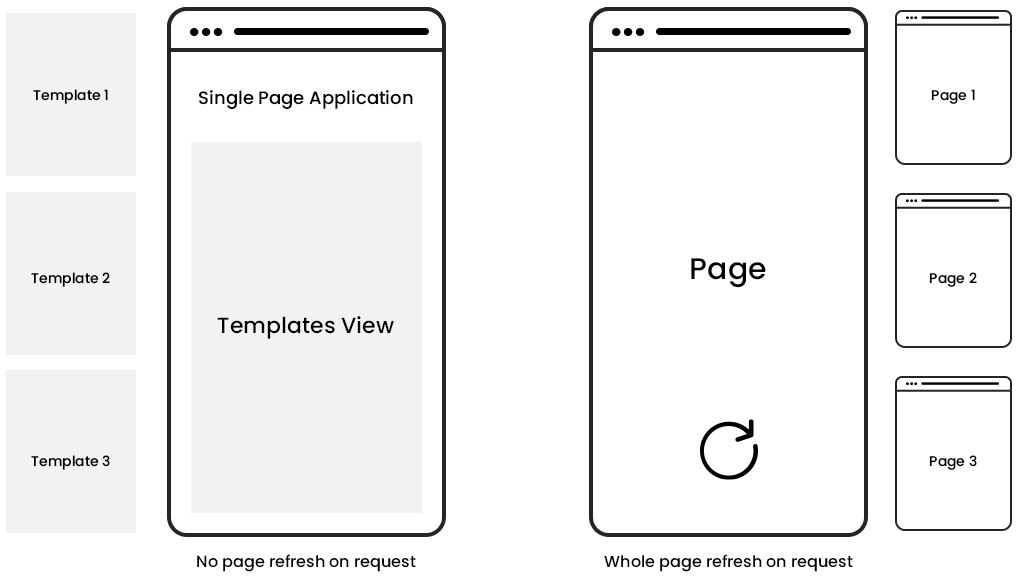
\includegraphics[width=1.0\textwidth]{spa-template}
    \caption{Views in Traditional Page and SPA[2].}
\end{figure} 

\bigskip
There are a lot of modern services that use SPA technology like facebook, airbnb, twitter, paypal, gmail or even netflix. The biggest benefits of this web application model are quick loading time, good caching abilities, improved user experiance or rapid front-end development. \\

\bigskip
Beyond usual frameworks dedicated for SPA services are
\begin{itemize}
	\item  Angular.js
	\item React.js
	\item Backbone.js
	\item Ember.js
\end{itemize}

It is no secret that preferable programming technology stack for such development would be JavaScript, TypeScript, HTML, CSS and some back-end in Java, Python or PHP. With that being said, WebToolkit library seems to be very unorthodox tool for this task. The whole development process starts and ends with C++ code, which makes it interesting and unusual.
\newpage

}
\subsection{WebToolkit Features}
{
\tab WebToolkit library has a lot to offer. Now of course - creating web application in low-level language comes with a prize. It's biggest disadvantage is that while programming we have no control of HTML code. There is also a necessity of re-compiling the code with every change introduced where there is no such need when using regular tools. However - compilation time is quite fast and the library implementation is very robust. 
\begin{figure}[h]
  \centering
    
\includegraphics[width=0.7\textwidth]{features}
    \caption{WebToolkit logo and features\cite{wtlogo}.}
\end{figure}

\subsubsection*{Core Library} 
{
\tab What is really important is that core library is fully open source and still under development. It's implementation allows to integrate it with 3rd party JavaScript libraries, which is a nice addition for developers that create services with more advanced front-end layer. What is more, WT is fully compatible with HTML5 and HTML4 browsers. Thus, as a hybrid single page framework it supports browser history navigation. The bottom line is, WT is a high performance library which is something you would expect from a C++ library. It is optimized when it comes to asynchronous I/O, multi-threading and throughout all rendering.

\bigskip
Event handling is completed with C++11 lambdas or bound object methods, which are a part of C++11 signal/slot API for responding to various events. Server-initiated updates are also available through WebSockets and automatic fallaback to AJAX. The handling itself is also completed with efficient synchronization of browser using session, which incrementally renders updates of application states. The concept of session is thoroughly described in implementation chapter.

\bigskip
Core library also provides 2D and 3D painting support to users and developers. Through WT API it is possible to generate simple graphics objects like HTML5 canvas, inline SVG or inline VML. Browser native vectors are also leveraged by rendering common image formats like PNG, GIF or even PDF. WT broads the variety of graphics support by also supporting hardware-accelerated 3D painting API like for instance server-side OpenGL.
}

\subsubsection*{Security}
{
\tab As a completed web-development library, WebToolkit provides built-in security layer to the applications which contains:

\begin{itemize}
	\item kernel-level memory protection in isolated sessions
	\item TLS/SSL support
	\item Cross-Site Scripting (XSS) prevention
	\item Request Forgery (CSRF) prevention
	\item Application logic attack prevention
	\item DoS mitigation
	\item \textbf{Authentication module} (including support for OAuth 2.0 and OpenID Connect)
\end{itemize}

\begin{figure}[h]
  \centering
    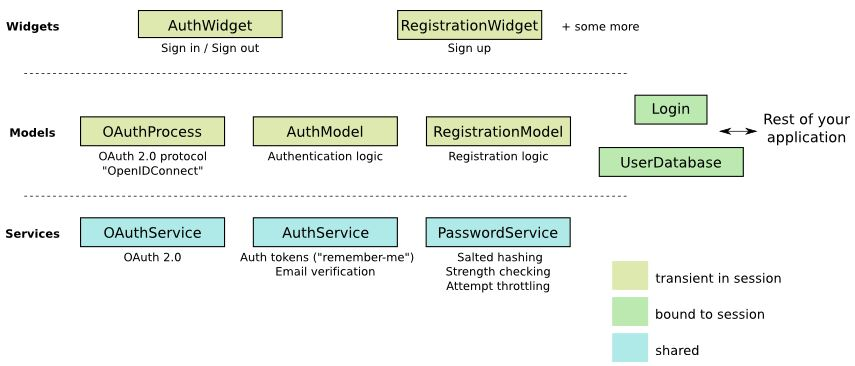
\includegraphics[width=1.1\textwidth]{auth-module}
    \caption{Main classes of the authentication module\cite{authmodule}.}
\end{figure}

The authentication module itself occurred to be significantly important and helpful in Web Banking Application. Some of the classes which implement basic user features are presented above. What it means is that secure and robust service functionalities like signing in/out, registration or authentication are already provided.

}

\subsubsection*{Database support}
{
\tab As any other modern library, WT supports databases with a sub-library called Wt::Dbo, which by implementing ORM (Object-Relational Mapper) becomes a convenient way to communicate C++ application with SQL databases. What is more, Wt::Dbo as a self-contained sub-library is independent from Wt itself, which means it could be used for standalone back-end service. Other basic Wt::Dbo features are: 

\begin{itemize}
	\item Support for
	\begin{itemize}
     \item Sqlite3
     \item Firebird
     \item MariaDB
     \item MySQL
     \item SQL Server
     \item PostgreSQL
     \end{itemize}
	\item Native SQL to query objects and fields
	\item Session with first-level cache
	\item DB transactions
	\item CRUD operations
	\item Many-to-One and Many-to-Many relations
	\item Just C++ without XMLs or Macros

\end{itemize}
}

\subsubsection*{Deployment}
{
\tab Extremely important thing in any application is process of Deployment. WT through various abstract interfaces connects with outer world. The basic one is built-in httpd but among others:

\begin{itemize}
	\item Built-in \textbf{HTTPD}
	\begin{itemize}
     \item Simple and high performance with multithreading and asynchronous I/O based on C++ asio library
     \item Supports WebSockets and HTTP(s) with chunking and compression
     \item Available for many platforms like Linux, Windows and any UNIX like systems
     \end{itemize}
	\item \textbf{FASTCGI}
	\begin{itemize}
     \item Integrated with common web servers like apache
     \item Supported for Linux and UNIX
     \end{itemize}
	\item \textbf{ISAPI}
	\begin{itemize}
     \item Integrated with Microsoft IIS server
     \item Completed with asynchronous API
     \item Supported for Windows
     \end{itemize}
\end{itemize}
}
\newpage
}

\subsection{Hello World Application}
{
Lets go through simple Hello World applications just to get in touch with WebToolkit library environment.

\begin{lstlisting}[frame=single, basicstyle=\small, language=C++, caption={A complete "Hello world" application \cite{helloworldapp}}, captionpos=b]
#include <Wt/WBreak.h>
#include <Wt/WContainerWidget.h>
#include <Wt/WLineEdit.h>
#include <Wt/WPushButton.h>
#include <Wt/WText.h>

class HelloApplication : public Wt::WApplication
{
public:
    HelloApplication(const Wt::WEnvironment& env);

private:
    Wt::WLineEdit *nameEdit_;
    Wt::WText *greeting_;
};

HelloApplication::HelloApplication(const Wt::WEnvironment& env)
    : Wt::WApplication(env)
{
    setTitle("Hello world");

    root()->addWidget(std::make_unique<Wt::WText>("Your name, please? "));
    nameEdit_ = root()->addWidget(std::make_unique<Wt::WLineEdit>());
    
    Wt::WPushButton *button = 
    	root()->addWidget(std::make_unique<Wt::WPushButton>("Greet me."));
    	
    root()->addWidget(std::make_unique<Wt::WBreak>());
    greeting_ = root()->addWidget(std::make_unique<Wt::WText>());
    
    auto greet = [this]{
      greeting_->setText("Hello there, " + nameEdit_->text());
    };
    button->clicked().connect(greet);
}

int main(int argc, char **argv)
{
    return Wt::WRun(argc, argv, [](const Wt::WEnvironment& env) {
      return std::make_unique<HelloApplication>(env);
    });
}
\end{lstlisting}

\newpage
Now when it comes to building, it could be done locally by setting up a localhost HTTP server. Having IDE set-up it is done automatically. Otherwise while operating on UNIX-like systems:

\begin{lstlisting}[frame=single, basicstyle=\small, language=C++, caption={Building "Hello world" application}, captionpos=b]
$ g++ -std=c++14 -o hello hello.cc -lwthttp -lwt
$ ./hello --docroot . --http-address 0.0.0.0 --http-port 9090
\end{lstlisting}

\bigskip
The final result is:
\begin{figure}[h]
  \centering
    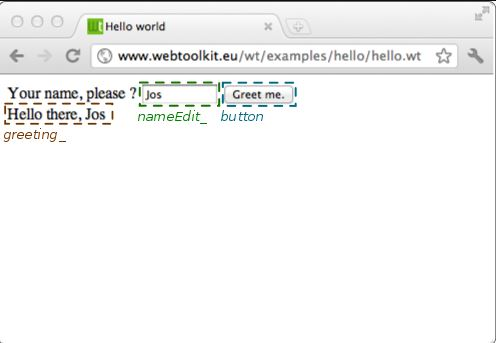
\includegraphics[width=0.7\textwidth]{hello-app}
    \caption{Hello Application on WT.}
\end{figure}

\bigskip
The above code presents basic concepts of the library workflow.

\begin{labeling}{alligator}
\item [\textbf{class HelloApplication}] A class that represents application and extends Wt::WApplication. Contains ctor that takes Wt::WEnvironment and private fields that represents input field and output greeting string wrapped in Wt::WText,
\item [\textbf{LINE 20:}] Sets title of appliaction which will be visible in web browser's card,
\item [\textbf{LINE 22-29:}] This part of the code handles adding widgets to the root which represents a container for the widgets. This is an implementation of SPA concept where we create widgets and plug them in or out, for instance by addWidget() function,
\item [\textbf{LINE 31:}] Lambda expression that returns WText string which called upon clicking the button,
\item [\textbf{LINE 34:}] Calling lambda expression from line 31 when button is clicked,
\item [\textbf{MAIN:}] Creating and running application.
\end{labeling} 


}
\subsection{Widgets gallery}
\section{DevOps layer}
\subsection{Distributed version-control system}}
\subsubsection{GitHub}
\subsection{Proprietary issue tracking}
\subsubsection{JIRA Software}
\subsection{Other Atlassian tools}
\subsection{Containers}
\subsubsection{Docker}
\subsubsection{Containers vs OS-level virtualization}
\subsection{Automation server}
\subsubsection{GitHub CMake workflows}
\paragraph{Example CMake file used in project}
\begin{verbatim}
CMAKE_MINIMUM_REQUIRED(VERSION 2.4)
Project(ConsoleApplication1)

# If Visual Studio IDE
IF(MSVC_IDE)
	# Copy user file
  FILE(COPY ${CMAKE_CURRENT_SOURCE_DIR}/${PROJECT_NAME}.vcxproj.user DESTINATION ${CMAKE_CURRENT_BINARY_DIR})
ENDIF(MSVC_IDE)

# If Eclipse IDE
IF(${CMAKE_EXTRA_GENERATOR} MATCHES ".*Eclipse.*")
	IF(${CMAKE_BUILD_TYPE} STREQUAL "Debug")
		# Copy debug user file
    FILE(COPY ${CMAKE_CURRENT_SOURCE_DIR}/${PROJECT_NAME}-debug.exe.launch DESTINATION ${CMAKE_CURRENT_BINARY_DIR})
	ENDIF()
	IF(${CMAKE_BUILD_TYPE} STREQUAL "Release")
		# Copy release user file
    FILE(COPY ${CMAKE_CURRENT_SOURCE_DIR}/${PROJECT_NAME}-release.exe.launch DESTINATION ${CMAKE_CURRENT_BINARY_DIR})
	ENDIF()
ENDIF()

# Copy resources to build tree
# FILE(COPY ${CMAKE_CURRENT_SOURCE_DIR}/resources DESTINATION ${CMAKE_CURRENT_BINARY_DIR})

SET(ConsoleApplication1_SRC src/Main.cpp)

# If Visual Studio IDE
IF(MSVC_IDE)
	SET(ConsoleApplication1_SRC ${ConsoleApplication1_SRC} src/Main.cpp)
ENDIF(MSVC_IDE)

ADD_EXECUTABLE(ConsoleApplication1 ${ConsoleApplication1_SRC})

ADD_SUBDIRECTORY("wt-4.3.1/" "Wt 4.3.1 msvs2019 x64/lib/")
# Set Wt include and library paths
INCLUDE_DIRECTORIES("Wt 4.3.1 msvs2019 x64/include/")

INCLUDE_DIRECTORIES("include")
FILE(GLOB SOURCES "src/*.cpp")
ADD_EXECUTABLE(ConsoleApplication1 ${SOURCES})
TARGET_LINK_DIRECTORIES(ConsoleApplication1 PUBLIC "Wt 4.3.1 msvs2019 x64/lib/")

TARGET_LINK_LIBRARIES(ConsoleApplication1
  debug wtd optimized wt
  debug wthttpd optimized wthttp
  debug wtdbod optimized wtdbo
  debug wtdbosqlite3d optimized wtdbosqlite3
  )
\end{verbatim}
\subsubsection{CircleCI}
\subsection{Doxygen docs}

\section{Implementation}
\subsection{Server side session}
\subsection{Logging panel}
\subsection{Database}
\subsection{User features}
\subsubsection{Transferring money}
\subsubsection{Checking user balance}
\subsection{Admin features}
\subsubsection{Listing all users}
\subsubsection{Access to server logs}
\subsection{Modern C++ features}

\section{Testing}
\subsection{Unit testing}
\subsection{Regression testing}
\section{Summary}
\section{Literature}
{

\begin{thebibliography}{9}

\bibitem{cmakeintroduction}
  Introduction to CMake,
  \emph{http://derekmolloy.ie/hello-world-introductions-to-cmake}.
  
\bibitem{singlepageapplications}
  Single Page Applications,
  \emph{https://www.excellentwebworld.com/what-is-a-single-page-application}.
  
\bibitem{wtlogo}
  WT Logo and Features,
  \emph{https://www.webtoolkit.eu/wt/features}.

\bibitem{authmodule}
  Introduction to Wt::Auth,
  \emph{https://www.webtoolkit.eu/wt/doc/tutorial/auth.html}.
  
\bibitem{helloworldapp}
  Wt Hello World Application,
  \emph{https://www.webtoolkit.eu/wt/doc/tutorial/wt.html}.

\end{thebibliography}

\textbf{Additional materials} \begin{itemize}
	\item LaTeX wikibooks \newline \textit{https://en.wikibooks.org/wiki/LaTeX}

\end{itemize}

}
\newpage

\linespread{1.3}
\selectfont

\end{document}